\section{Udvælgelse af gestik-par til at justere lydstyrken}
\label{TestresultaterVolumen}
%
Udvælgelsen af hvilket gestik-par, der skal knyttes til at justere lydstyrken foretages på baggrund af testpersonernes begrundelser for til- og fravalg af de foreslåede gestikker. Der fokuseres først på hvilke gestik-par testpersonerne har inddraget i deres top tre rangering og i den forbindelse, om det er muligt at ekskludere nogle gestik-par. Derefter fokuseres der på testpersonernes begrundelser for, hvorfor de har valgt de gestik-par, som de har, hvorunder forbedringsforslag inkluderes, hvis testpersonerne fremsætter nogle. Afsnittet vil afslutningsvist ende ud i hvilket gestik-par, der vælges til at justere lydstyrken.\blankline
%
Få at få et overblik over, hvor ofte de ni forskellige gestik-par individuelt indgår på enten en første-, anden- eller tredjeplads i top tre rangeringen opstilles følgende \autoref{fig:SamletTopTreVolumen}.
%
\begin{figure}[H]
	\centering
	\includegraphics[resolution=300,width=0.9\textwidth]{Test1/DatabehandlingGrafer/TopTreVolumen}
	\caption{Søjlediagram over hvordan hvert gestik-par indgår i testpersonernes top tre i forhold til at justere lydstyrken. Data forefindes i \autoref{app:TopTreRangeringVolumen}.}
	\label{fig:SamletTopTreVolumen}
\end{figure}
\noindent
%
På \autoref{fig:SamletTopTreVolumen} fremgår det tydeligt, at GP2, GP3 samt GP4 er de tre gestik-par, som uafhængigt af den specifikke plads, indgår flest gange i testpersonernes top tre. Efterfulgt af GP1, GP5 og GP9. Derudover tyder det på, at hverken GP6, GP7 eller GP8 er specielt eftertragtet, da de henholdvis kun indgår fire, aldrig og to gange i testpersonernes samlede top tre, jævnfør \autoref{fig:SamletTopTreVolumen}. For at vurdere om der er belæg for, at ekskludere et eller flere gestik-par opstilles følgende \autoref{fig:DaarligstGestikVolumen}. 
%
\begin{figure}[H]
	\centering
	\includegraphics[resolution=300,width=0.9\textwidth]{Test1/DatabehandlingGrafer/FravalgtVolumen}
	\caption{Søjlediagram over hvilke gestik-par testpersonerne fravælger i forbindelse med at justere lydstyrken.}
	\label{fig:DaarligstGestikVolumen}
\end{figure}
\noindent
%
På \autoref{fig:DaarligstGestikVolumen} opsummeres antallet af gange hvert gestik-par fravælges af testpersonerne. Da otte ud af 18 testpersoner har fravalgt GP7 konkluderes det, at testpersonerne ikke bryder sig om GP7, hvorfor GP7 ekskluderes. På \autoref{fig:SamletTopTreVolumen} fremgår det, at GP8 hverken tildeles en første- eller andenplads og derudover kun indgår to gange på en tredjeplads og da GP8 fravælges af fire testpersoner, så vurderes det, at GP8 er overflødig og irrelevant. Der er derfor belæg for at ekskludere GP8. Tilsvarende er gældende for GP6, som kun indgår fire gange i testpersonernes samlede top tre og kun tildeles en førsteplads én gang, jævnfør \autoref{fig:SamletTopTreVolumen}, og derudover fravælges to gange, jævnfør \autoref{fig:DaarligstGestikVolumen}. Der er derfor belæg for at ekskludere GP6. I \autoref{app:TestresultaterVolumenDaarlig} forefindes en dybere analyse af hvorfor testpersonerne fravælger de gestik-par, som de gør. 

Ekskluderingen af de tre gestik-par medfører, at den efterfølgende analyse vil omhandle testpersonernes begrundelser for at vælge GP1, GP2, GP3, GP4, GP5 samt GP9.
%
\subsection{Testpersonernes begrundelse for valg af gestik-par 1}
\label{TestresultaterValgAfGestikkerBegrundelseGP1Volumen}
%
Med udgangspunkt i \autoref{fig:SamletTopTreVolumen} tildeles GP1 en førsteplads af to testpersoner, en andenplads af tre testpersoner og en tredjeplads af én testperson. GP1 illustreres på \autoref{fig:GestikPar1Volumen}. De testpersoner, som har tildelt GP1 en førsteplads, begrunder det med at det er en velkendt bevægelse; at dreje på en knap for at skrue op. Derudover påpeger TP8 både at bevægelsen i GP1 er tydeligere sammenlignet med GP2 og at GP1 er naturlig. I tillæg påpeger TP16, at bevægelsen i GP1 så mere behagelig ud sammenlignet med GP2, som testpersonen fandt ukomfortabel. 

En af årsagerne til at TP16 vurderer at GP2 er ukomfortabel skyldes formentlig, at i videooptagelsen bliver GP2 ikke gengivet lige så afslappet, som det var hensigten. I videooptagelsen fremgår det at hele armen skal i bevægelse; fra skulderen og ud til fingrene, hvilket ikke er hensigten med GP2. Hensigten med GP2 er derimod at bevægelsen dannes ud fra en kombination mellem underarm, håndled og fingre, så det tilnærmelsesvist er den samme bevægelse, som ved GP1. Sammenholdes TP16's udsagn med testpersonens bevægelser, når testpersonen opfordres til at fremsætte et forbedringsforslag, så gengiver TP16 GP2 og det er først når testlederen konfronterer TP16, at testpersonen gengiver GP1. Afslutningsvist gengiver TP16 ikke GP1, men noget der tilnærmelsesvist minder om GP2 bortset fra, at fingrene er udstrakt og roteres i en cirkulærbevægelse. Da hverken testpersonens udsagn eller bevægelser stemmer overens med GP1, så indikerer det at TP16 formentligt foretrækker noget, der i højere grad minder om GP2, men særligt foretrækkes en cirkulærbevægelse.
%
\begin{figure}[H]
	\centering
	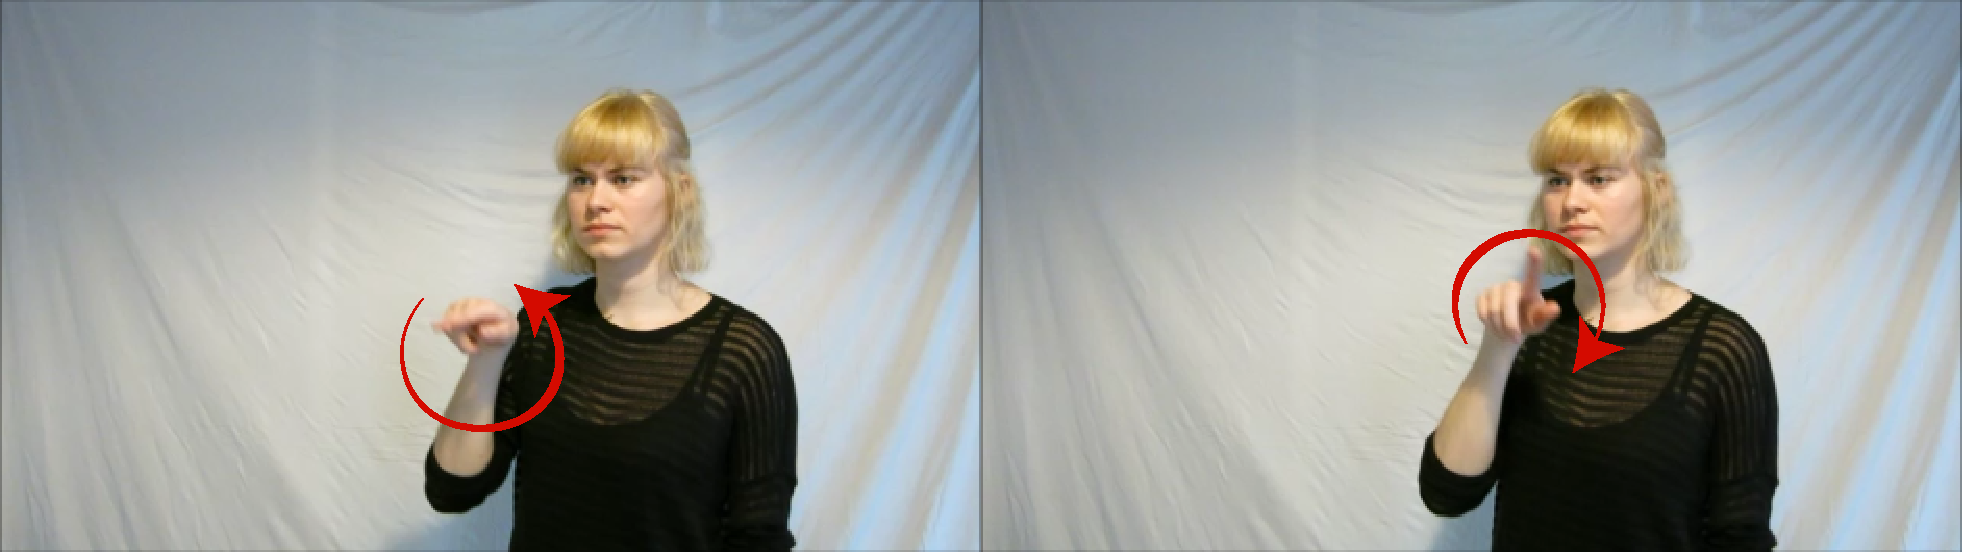
\includegraphics[resolution=300,width=0.9\textwidth]{Test1/Gestik-par/Gestik1_Volumen}
	\caption{Illustration af gestik-par 1; cirkulærbevægelse med pegefingeren i urets retning for at skrue op og mod uret for at skrue ned.}
	\label{fig:GestikPar1Volumen}
\end{figure}
\noindent
%
Da der kun er to testpersoner, som har tildelt GP1 en førsteplads og det er begrænset hvilke egenskaber de foretrækker ved GP1, vurderes det, at det er nødvendigt at inddrage de resterende fire testpersoner, som har inkluderet GP1 i deres top tre. De testpersoner, som har tildelt GP1 en anden- eller tredjeplads, begrunder det ud fra en kombination af følgende egenskaber: 
%
\begin{multicols}{3}
    \begin{itemize}
        \item Naturlig bevægelse
        \item Intuitiv 
        \item Nem at forstå
        \item Universel
        \item Nem
        \item Overskuelig
        \item Cirkulærbevægelse
        \item Kræver én hånd
\end{itemize}
\end{multicols}
\noindent
%
Derudover kommenterer TP4, at både GP1 og GP2 er gestikker, der kan forbindes direkte til at justere lydstyrken. Ifølge TP5 kan bevægelsen i GP1 gengives overalt samt i forskellige størrelser. Selvom TP5 ikke inkluderer GP2 i sin top tre, så giver TP5 alligevel udtryk for godt at kunne lide, hvad testpersonen definerer som volumenknappen, svarende til GP2. Årsagen til at GP2 ikke indgår i TP5's top tre skyldes, ifølge testpersonen, at GP2 er langsom at gengive sammenlignet med GP1. Fælles for både TP9 og TP13 er, at de begge foretrækker gestikker, hvor det kun kræver én hånd at gengive dem. Derudover kommenterer TP13 at cirkulærebevægelser er sjove og at de minder om en knap, hvilket ligeledes er gældende for GP2.      
%
\subsection{Testpersonernes begrundelse for valg af gestik-par 2}
\label{TestresultaterValgAfGestikkerBegrundelseGP2Volumen}
%
Med udgangspunkt i \autoref{fig:SamletTopTreVolumen} tildeles GP2 en førsteplads af fire testpersoner, en andenplads af to testpersoner og en tredjeplads af tre testpersoner. GP2 illustreres på \autoref{fig:GestikPar2Volumen}. De fire testpersoner, som har tildelt GP2 en førsteplads, begrunder det ud fra en kombination af følgende egenskaber: 
%
\begin{multicols}{3}
    \begin{itemize}
        \item Naturlig bevægelse
        \item Giver mening
        \item Intuitiv 
        \item Nem at huske
        \item Behageligt at dreje
        \item Cirkulærbevægelse
        \item Kræver én hånd
        \item Specifik
\end{itemize}
\end{multicols}
\noindent
%
Ifølge TP1, så tænkte testpersonen på GP2 før testpersonen blev præsenteret for gestik-parret. Som tidligere nævnt, vælger TP14 gestikker ud fra hvad der ikke naturligt forekommer, når testpersonen normaltvist gestikulerer, hvorfor TP14 tildeler GP2 førstepladsen. Lignende argumenter fremsættes af TP18, som påpeger at fordi bevægelsen i GP2 er så specifik, så er det ikke en bevægelse der fejlagtigt gengives. 
%
\begin{figure}[H]
	\centering
	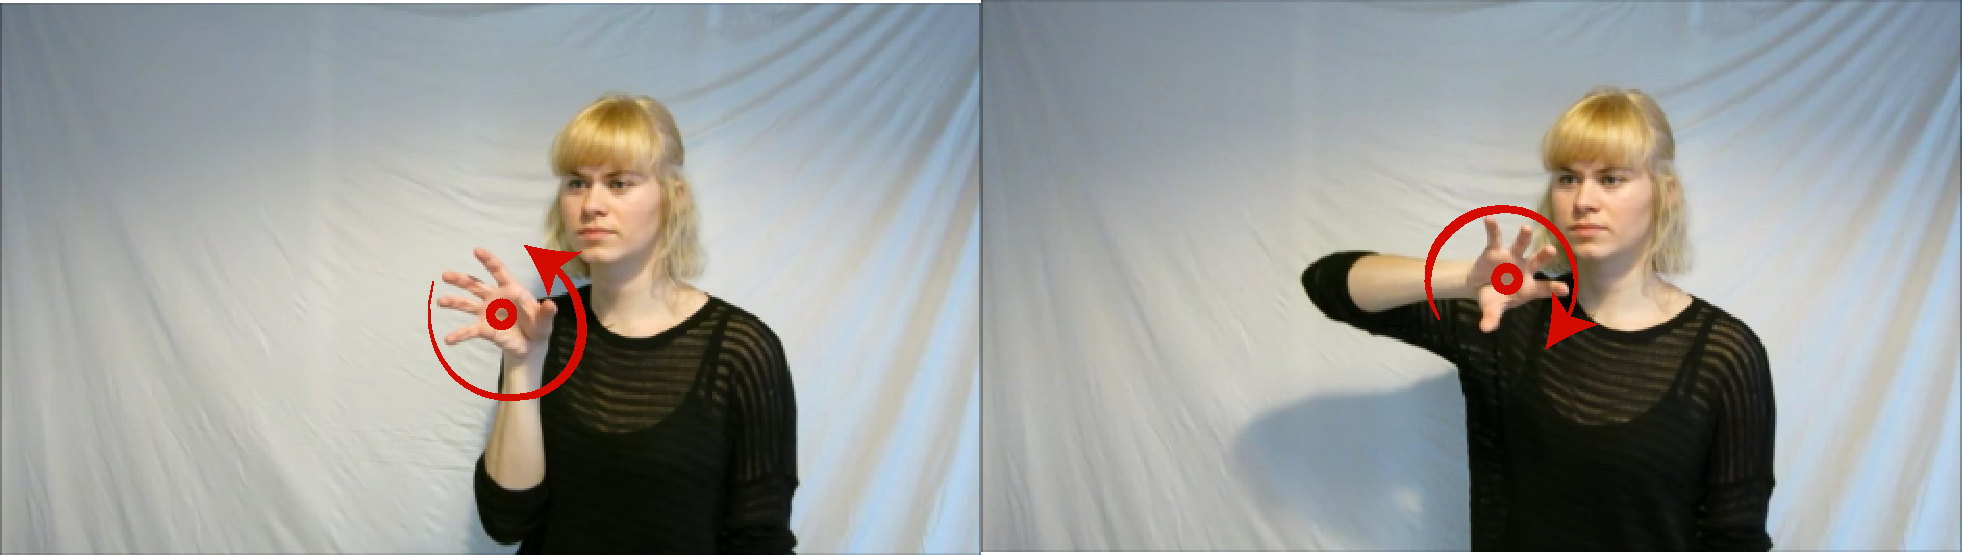
\includegraphics[resolution=300,width=0.9\textwidth]{Test1/Gestik-par/Gestik2_Volumen}
	\caption{Illustration af gestik-par 2; cirkulærbevægelse med halv bøjede fingrene, ligesom hvis det var en dreje-knap, der blev brugt. Der skal drejes med uret for at skrue op og mod uret for at skrue ned.}
	\label{fig:GestikPar2Volumen}
\end{figure}
\noindent
%






 . Ifølge testperson 9 fravælges gestik-par 2 fordi bevægelsen var stor og klodset, hvilket indikerer at hensigten med gestik-parret igen er fejlfortolket.

Seks ud af de ni testpersoner, som har inkluderet gestik-par 2 i sin top tre, forbinder gestikken med en drejeknap, som de i forvejen er vant til at interagere med for at skrue op eller ned på et anlæg, jævnfør \autoref{fig:GestikPar2Volumen}. 


Udover at bevægelsesmængden i gestik-par 2 ikke behøver, at være så udtryksfuld, som det blev illustreret i videooptagelser, så er det kun to testpersoner, som har forbedringsforslag. Testperson 14 foreslår, at den ikke-dominante hånd, altså hånden, som ikke skal foretage cirkelbevægelsen, inkluderes, så det kræver begge hænder at skrue op og ned. I og med at størstedelen af testpersonerne foretrækker gestikker, som kun kræver én hånd, afvises foreslaget, men det tages til eftertrakning, at der måske skal være et nyt element i gestik-par 2. Et forslag til det fremsættes af testperson 1, som foreslår at hånden først er lukket sammen i en knytnæve og når hånden åbnes, så kan bevægelserne i gestik-par 2 udføres. Det nye element i gestik-par 2 behøver ikke nødvendigvis at være en lukket knytnævne, men kan være en indikation af, at brugeren tager fat i en drejeknap, da flere testpersoner forbinder gestik-par 2 med dette. Fordelen ved at implementere en indikation af, at brugeren tager fat i en drejeknap er, at teknologien i musikanlægget højst sandsynligt vil have nemmere ved at genkende hvilken ændring af volumen brugeren ønsker, hvis der laves en indikation af funktionen før volumen ændres på. 

En af fordelene ved at vælge gestik-par 2 fremfor gestik-par 1 er, at gestik-par 2 oftere indgår i testpersonernes samlede top tre, jævnfør \autoref{tab:GestikParITopTreVolumenOversigt}. Det anses ydermere for at være en fordel, at flere testpersoner forbinder bevægelsen i gestik-par 2 med noget de i forvejen er vant til, fordi de så ikke nødvendigvis behøver at lære noget nyt. Derudover antages det, at størstedelen af de personer, som har \textit{high-end} lydudstyr formentlig også har en forstærker, hvorpå lydstyrken normalvist ændres ved at dreje på en drejeknap, hvilket formentlig vil gøre det lettere for brugeren, at koble gestik-par 2 til den funktion. Ydermere påpeger både testperson 14 og testperson 18, at bevægelsen i gestik-par 2 ikke er en bevægelse, der normalvist indgår i ens naturlige gestikulation. Med forbehold for, at gestik-par 2 ikke nødvendigvis skal gengives på præcis samme måde, som det fremgår i videooptagelsen og at der muligvis først skal være en indikation af, at nu skal der skrues op eller ned, så vurderes det, at gestik-par 2 egner sig bedre end gestik-par 1 til at skrue op og ned.
%
\begin{figure}[H]
	\centering
	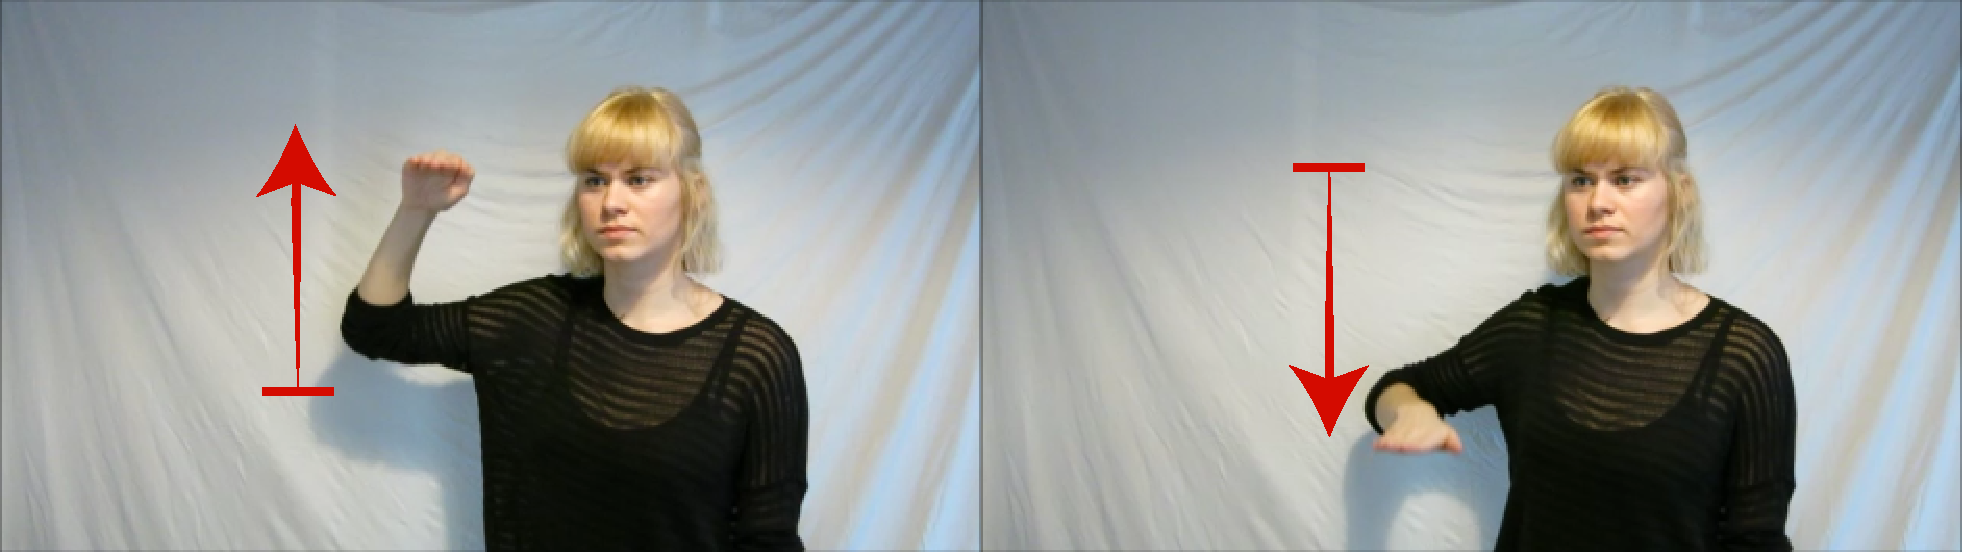
\includegraphics[resolution=300,width=0.9\textwidth]{Test1/Gestik-par/Gestik3_Volumen}
	\caption{Illustration af gestik-par 3; horisontal hånd løftes vertikalt med håndfladen nedad for at skrue op og for at skrue ned sænkes hånden vertikalt med håndfladen nedad.}
	\label{fig:GestikPar3Volumen}
\end{figure}
\noindent
%
På \autoref{fig:SamletTopTreVolumen} fremgår det, at gestik-par 3 er det gestik-par, som sammenlagt indgår flest gange i testpersonernes top tre; 12 gange i alt. Gestik-par 3 illustreres på \autoref{fig:GestikPar3Volumen}. Det tyder på, at ligesom ved de to foregående gestik-par, så foretrækker de testpersoner, som har tildelt gestik-par 3 en første plads, ligeledes at bevægelsen kan gøres med én hånd. Testperson 4 har tildelt gestik-par 3 en første plads ud fra, hvad der passede godt til det testpersonen valgte til pause og start, hvilket var gestik-par 1, jævnfør \autoref{fig:GestikPar1Volumen}. I og med at det gestik-par blev sorteret fra til pause og start, så er det ikke sikkert, at testpersonen stadig vil tildele gestik-par 3, til at skrue op og ned, en første plads. Testperson 10 giver, foruden at gestik-par 3 er intuitiv og nem at huske, udtryk for, at bevægelsen passer godt til det den skal gøre. Lignende tendens går igen ved testperson 11; som foruden at vurdere gestik-par 3 som værende både logisk og intuitiv, giver udtryk for, at hvis der skal skrues op, så bør det være med en opadgående bevægelse. Ifølge testperson 6 er både gestik-par 3 og gestik-par 4 naturlige og nemmere at udføre, i forhold til hvis der skal være en bestemt reference, som der blandt andet er i gestik-par 5, jævnfør \autoref{fig:GestikPar5Volumen}. Testperson 13 har svært ved uddybe hvorfor gestikkerne er rangeret i den rækkefølge, som fremgår af \autoref{tab:GestikParITopTreVolumen}, men testpersonen giver udtryk for godt, at kunne lide de gestik-par, hvor hånden enten skal hæves eller sænkes for at skrue op og ned. Både testperson 6 og testperson 13 giver udtryk for, at det er nemt at udføre bevægelserne i gestik-par 3. I tillæg kommenterer testperson 15, at gestik-par 3 er simpel. 

Disse synspunkter går igen ved testperson 12, som har tildelt gestik-par 3 en anden plads, jævnfør \autoref{tab:GestikParITopTreVolumen}. Ydermere giver testperson 16 og testperson 1 udtryk for, at gestik-par 3 giver mening. Dog tyder det på, at testperson 16 ikke kan huske sin top tre, da testpersonen bliver nødt til at spørge testlederen. Testperson 1, som har tildelt gestik-par 3 en tredje plads, forbinder gestikken med hvordan lyd visualiseres på en computer, hvor testperson 8 giver udtryk for, at det er den gestik, der bruges til at dirigere et kor. Ifølge testperson 7, så har testpersonen tildelt gestik-par 3 en tredje plads, fordi gestik-parret er en kombination af gestik-par 5, jævnfør \autoref{fig:GestikPar5Volumen}, og gestik-par 9, jævnfør \autoref{fig:GestikPar9Volumen}, i forhold til hvor meget kontrol testpersonen har. Testperson 17 kommenterer ikke på hvorfor gestik-par 3 indgår i top tre rangeringen.

Ud af de seks testpersoner, som har tildelt gestik-par 3 en første plads, er der ingen af dem, der begår fejl når de gengiver bevægelsen. Udover at bevægelserne gerne må udføres mere afslappet end hvad der er gengivet på \autoref{fig:GestikPar3Volumen}, så har ingen testpersoner forbedringsforslag. Baseret på foregående analyse vedrørende gestik-par 3, der illustreres på \autoref{fig:GestikPar3Volumen}, så er der på nuværende tidspunkt ikke belæg for, at ekskludere dette gestik-par.
%
\begin{figure}[H]
	\centering
	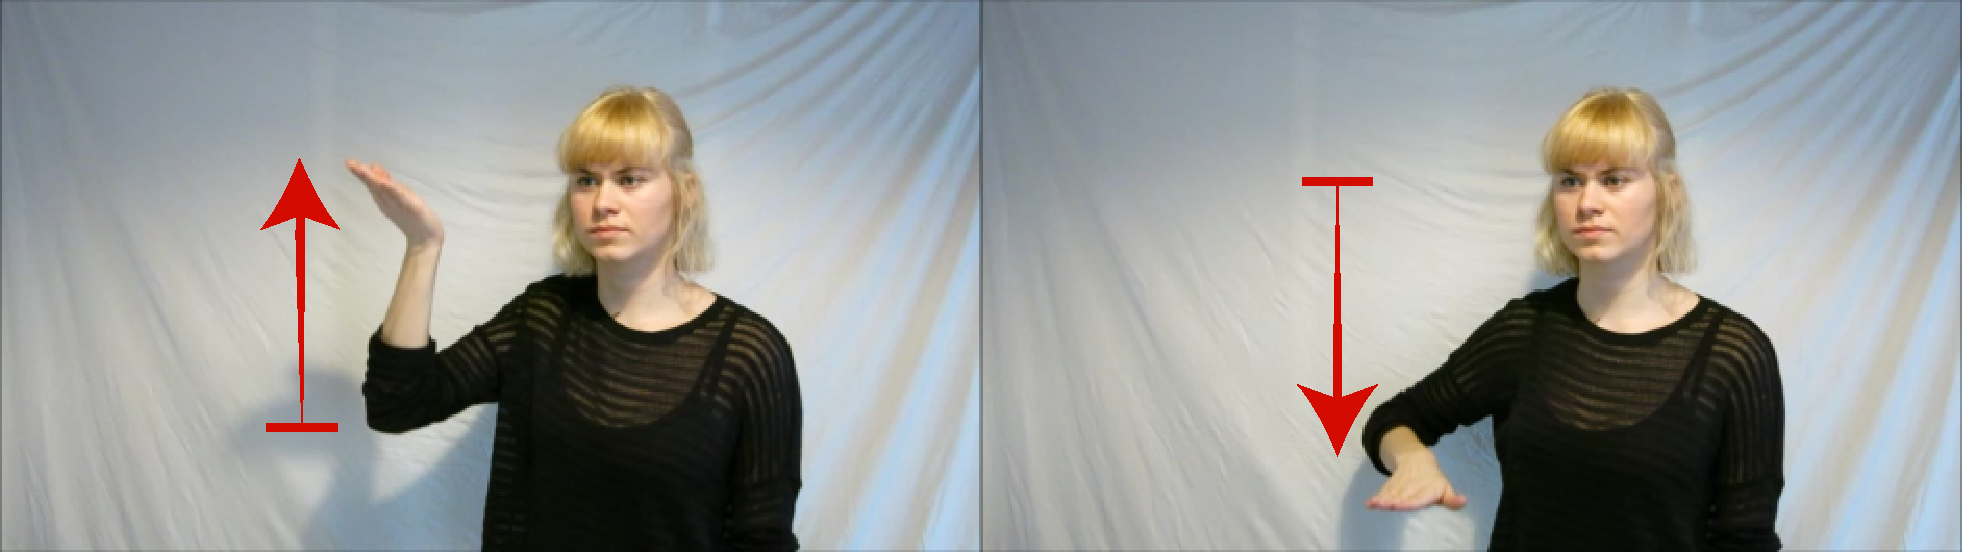
\includegraphics[resolution=300,width=0.9\textwidth]{Test1/Gestik-par/Gestik4_Volumen}
	\caption{Illustration af gestik-par 4; horisontal hånd løftes vertikalt med håndfladen opad for at skrue op og for at skrue ned sænkes hånden vertikalt med håndfladen nedad.}
	\label{fig:GestikPar4Volumen}
\end{figure}
\noindent
%
To ud af tre testperson, som har tildelt gestik-par 4 en første plads, giver udtryk for at bevægelsen giver mening. Gestik-par 4 illustreres på \autoref{fig:GestikPar4Volumen}. Testperson 2 begrunder yderligere sit valg med, at der er en tydelig indikation af hvad der er op og ned.  I tillæg kommenterer testperson 2, at gestik-par 4 er simpel, hvilket testperson 18 ligeledes giver udtryk for. Testperson 18 giver ydermere udtryk for, at årsagen til at gestik-par 4 er på en første plads skyldes, at armen ikke skal være på en bestemt måde, men bare løftes op eller ned. Som tidligere nævnt giver testperson 12 udtryk for, at foretrække gestikker, der kun kræver én hånd, hvilket ligeledes gør sig gældende ved gestik-par 4, jævnfør \autoref{fig:GestikPar4Volumen}. 

Fire ud af fem testperson, som har tildelt gestik-par 4 en anden plads, kommenterer, at det minder om gestik-par 3, jævnfør \autoref{fig:GestikPar3Volumen}. Dog kommenterer testperson 11 og testperson 15 henholdsvis, at der ikke bør skelnes mellem gestik-par 3 og gestik-par 4 og at gestik-par 4 er mere kompliceret end gestik-par 3. Derudover giver testperson 3 udtryk for, at det giver meningen at løfte et eller andet op, i det her tilfælde lydstyrken, og derefter skubbe det ned igen, hvorfor en lodret bevægelse giver mest mening. Ydermere beskriver testperson 11 og testperson 15 gestik-par 4 med ord som; intuitiv, logisk og simpel. Den eneste testperson, som har tildelt gestik-par 4 en trejde plads, er testperson 9. Testpersonen sammenligner gestik-par 4 med gestik-par 9, som illustreres på \autoref{fig:GestikPar9Volumen}. Derudover lægger testperson 9 vægt på hvad der er mindst krævende og mindst distraherende. 

Med udgangspunkt i på testpersonernes udsagn og at gestik-par 4 indgår ni gange i testpersonernes samlede top tre rangering, jævnfør \autoref{tab:GestikParITopTreVolumenOversigt}, så forefinder der på nuværende tidspunkt ikke belæg for, at ekskludere dette gestik-par.  
%
\begin{figure}[H]
	\centering
	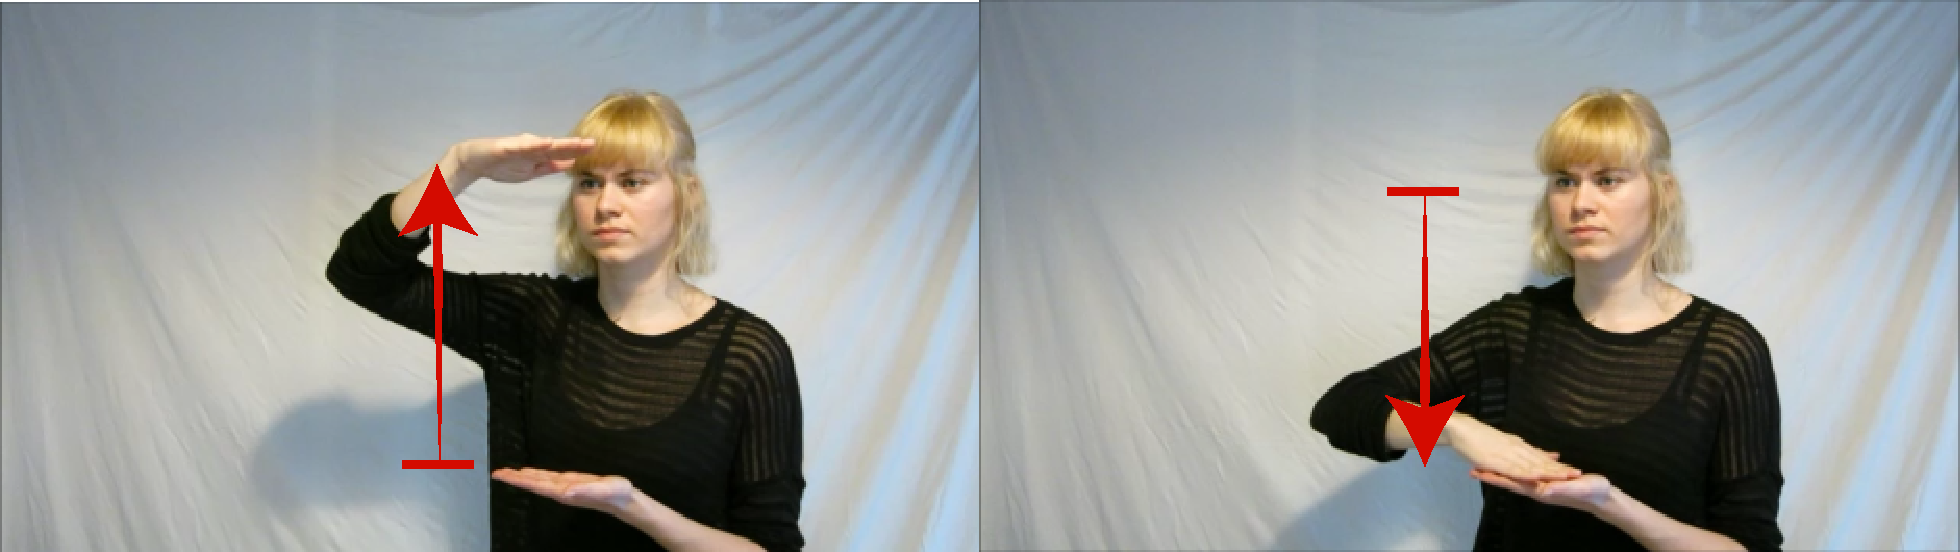
\includegraphics[resolution=300,width=0.9\textwidth]{Test1/Gestik-par/Gestik5_Volumen}
	\caption{Illustration af gestik-par 5; horisontal ikke-dominant hånd med håndfladen opad holdes stationær, mens den dominante hånd ligeledes holde horisontal med håndfladen nedad men løftes vertikalt væk fra den ikke-dominante hånd for at skrue op og sænkes mod den ikke-dominante hånd for at skrue ned.}
	\label{fig:GestikPar5Volumen}
\end{figure}
\noindent
%
Fra \autoref{fig:SamletTopTreVolumen} fremgår det, at gestik-par 5 ikke tildeles en første plads én eneste gang. Gestik-par 5 illustreres på \autoref{fig:GestikPar5Volumen}. Ifølge testperson 5, så er det nemmere, at kontrollere hvor meget lydstyrken skal ændres, hvis gestikken indeholder to hænder. Lignende kommer til udtryk ved testperson 7. Dog påpeger testperson 5, at testpersonen føler sig mere udsat ved gestik-par 5 sammenlignet med gestik-par 6, som er den samme bevægelse bare horisontalt. Foruden det testperson 10 og testperson 12 har givet udtryk for ved gestik-par 3, så præciserer de ikke nærmere hvorfor de har inkluderet gestik-par 5. Lignende går igen ved testperson 2, som heller ikke præciserer sit valg nærmere. 

Som nævnt tidligere, så foretrækker størstedelen af testpersonerne én-hånds gestikker, hvilket i sig selv er et godt argument for, at ekskludere gestik-par 5. Derudover indgår gestik-par 5 sammenlagt kun seks gange i testpersonernes samlet top tre og aldrig på en første plads, jævnfør \autoref{tab:GestikParITopTreVolumenOversigt}. Ydermere påpeger testperson 6 et potentielt problem ved gestik-par 5; hvis gestikken startes på den lydstyrke, som musikken allerede spiller ved, svarende til at hænderne er samlet, når der så skrues op øges afstanden mellem hænderne og når der skrues ned igen, så ender lydstyrken på hvad den oprindeligt var. Så hvis testpersonen gerne vil skrue endnu mere ned, så opstår der tvivl i hvordan det gøres; skal den dominante hånd så være referencen, mens den ikke-dominante hånd angiver hvor meget der skrues ned. Tages alt dette i betragtning vurderes det, at der er belæg for at ekskludere gestik-par 5.      
%
\begin{figure}[H]
	\centering
	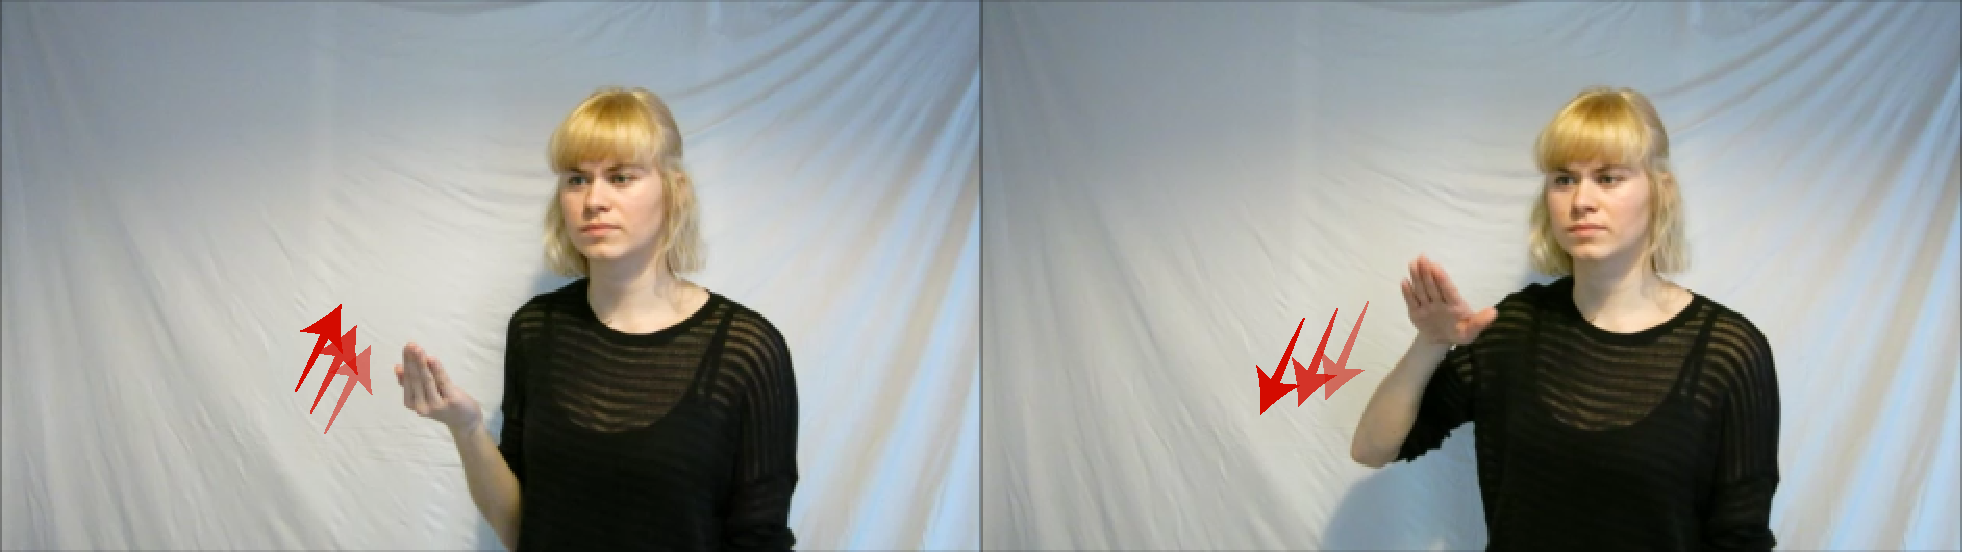
\includegraphics[resolution=300,width=0.9\textwidth]{Test1/Gestik-par/Gestik9_Volumen}
	\caption{Illustration af gestik-par 9; \enquote{Kom så}-bevægelse med fingrene for at skrue op og \enquote{Ro på}-bevægelse med fingrene for at skrue ned.}
		\label{fig:GestikPar9Volumen}
\end{figure}
\noindent
%
Den gennemgående tendens for, at testpersonerne vælger gestik-par 9 er, at den er smart. Gestik-par 9 illustreres på \autoref{fig:GestikPar9Volumen}. De to testpersoner, som har tildelt gestik-par 9 en første plads, begrunder det yderligere med, at det ifølge testperson 3 er meget sejt og ifølge testperson 9 er det naturligt. At gestik-par 9 er naturlig giver testperson 17 ligeledes udtryk for. Derudover beskrives gestik-par 9, som værende; logisk, hurtig, simpel og nem. Endvidere har hverken testperson 3 eller testperson 9 givet udtryk for forbedringer til gestik-par 9, men i begge tilfælde har testpersonerne oprindeligt valgt et andet gestik-par ind til de gengiver bevægelserne og begge konkluderer, at gestik-par 9 skal tildeles første pladsen.

Med udgangspunkt i testpersonernes argumenation for hvorfor de har valgt gestik-par 9 og taget i betragtning af, at gestik-par 9 sammenlagt indgår seks gange i testpersonernes samlede top tre, jævnfør \autoref{tab:GestikParITopTreVolumenOversigt} samt at gestik-parret er fravalgt to gange, jævnfør \autoref{app:TestresultaterVolumenDaarlig}, så vurderes det, at der er belæg for at ekskludere gestik-par 9. Ydermere påpeger testperson 7, at ved gestik-par 9 er der ingen kontrol over lydstyrken, så det kan være hvilken som helst lydstyrke testpersonen ender på ved gestik-par 9. \blankline
%
Baseret på foregående analyse af hvilket semaforisk gestik-par, der skal knyttes til at skrue op og ned for musikken, er det ikke muligt, at udpege et enkelt gestik-par. Valget står mellem gestik-par 2, gestik-par 3 og gestik-par 4, illustreret på henholdvis \autoref{fig:GestikPar2Volumen}, \autoref{fig:GestikPar3Volumen} og \autoref{fig:GestikPar4Volumen}. Fordelen ved at vælge gestik-par 2 er, at det ikke er en bevægelse, som normalvist indgår i ens kropsprog, hvorfor det forventes at sandsynligheden for, at bevægelsen laves ved en fejl er mindre end ved både gestik-par 3 og gestik-par 4. En anden fordel ved at vælge gestik-par 2 er, at størstedelen af testpersonerne forbinder gestikken med noget de er vant til i forvejen; netop at skrue op og ned på et anlæg via en drejeknap. I denne sammenhæng vælges det derfor, at knytte gestik-par 2 til at skrue op og ned.   

